\documentclass[a4paper]{article}

\usepackage{amsmath}  % extra math features
\usepackage{booktabs}  % nice tables
\usepackage[margin=25mm]{geometry}
\usepackage{graphicx} % required for inserting images
\usepackage{hyperref} % clickable hyperlinks
\usepackage{multirow}  % pandas to_latex() uses this
\usepackage{siunitx}  % use for all units
\usepackage{subcaption}  % for subfigures

% hyperref settings for better looking links
\hypersetup{
  colorlinks=true,
  linkcolor=blue,
  urlcolor=blue,
}
    
\title{
  DRAFT: v1 \\
  Vibration Characterization of Babies\\
  Transported in Strollers and Cargo Bicycles\\
  \vspace{2mm}
  \large{Prepared for VeiligheidNL}
}
\author{Gabriele Dell'Orto \and Brecht Daams \and Riender Happee \and Jason K. Moore}

\begin{document}

\maketitle

\section*{\centering Notice}
%
\textbf{This is a draft report. The values and results must be considered
preliminary and may change as the analysis is refined and rechecked.}

\section*{\centering Acknowledgements}
%
Thomas Valk and Jesper Meijerink helped design and perform the experiments.
Georgios Papaioannou and Arjo Loeve gave advice on the experimental design and
analyses.

\section{Introduction}
%
This paper reports on the vibration experienced by infants of different ages
when transported in cargo bicycles and strollers. Vibration can be related to
discomfort and might lead to negative health consequences. However, the topic is
poorly addressed in scientific literature, and only a few studies focus on the
effect of vibration on babies. To measure the actual vibration transmitted to
the babies, we equipped three strollers and two cargo bicycles with inertial
measurement units (IMU) and conducted several experiments across different road
surfaces and travelling speeds, using dummies representing the size of 0, 3, and
9 months old babies. We present analysis in the time and frequency domains,
allowing us to compare vertical accelerations at the baby-seat interface, as
recommended by ISO-2631-1. We investigate the influence of different variables
on vibration, such as type of vehicle, baby seat, travelling speed, dummy size
and mass, and road surfaces.

\section{Methods}
%
\subsection{Experimental Methodology}
%
In this section, we describe the measurement equipment used and the protocol
followed during the experimental campaign.

\subsubsection{Description of Test Equipment}
%
We conducted the experimental campaign using three different strollers, two
cargo bicycles, and two baby seats, chosen for their popularity and/or
distinctive features. The test involved three baby dummies representative of
various ages (different sizes and masses).

\paragraph{Strollers}
%
\begin{description}
  \item[Maxi-Cosi Street Plus] Among the most popular brands, this stroller comes
  with a cot configuration (0-3 months) and a baby seat option. It has large
  wheels, with only a marginal suspension system.
  (\href{https://www.maxi-cosi.nl/kinderwagens/street-plus?color_swatch_id=5519}{Maxi-cosi website})
  \item[Stokke BABYZEN YOYO 0+] It is the smallest foldable stroller on the
  market, it has only a marginal suspension system and smaller wheels compared
  to the other strollers on the market. It can be considered the ideal choice
  for holidays, being one of the few buggies that can be taken as hand
  luggage on the plane.
  (\href{https://tinylibrary.nl/products/kinderwagen-babyzen-yoyo-0-plus}{Model
  rented for the experiment})
  \item[Bugaboo Fox 5] It is featured by large wheels, and a suspension system
  which makes it an all-terrain stroller (according to the manufacturer). It has
  a large puncture-proof tyres and an air-permeable mattress.
  (\href{https://www.bugaboo.com/nl-nl/speciale-aanbiedingen/bugaboo-fox-5-bassinet-and-seat-stroller-black-base-midnight-black-fabrics-midnight-black-sun-canopy-PV006272.html?gad_source=1&gclid=Cj0KCQiA1Km7BhC9ARIsAFZfEIuB-6fQPRl5KyIHVJtion5lyD_Z1Qn-IP3shWoB_HXFozM1ySTXNfgaAgzFEALw_wcB&gclsrc=aw.ds}{Bugaboo
  website})
\end{description}

\paragraph{Cargo Bicycles}
%
\begin{description}
  \item[Urban Arrow Bicycle] This is a popular electric cargo bicycle in The
  Netherlands. This vehicle has two inline wheels which makes it roll into the
  curve like a regular bicycle. It is featured by a long frame that can carry
  loads usually placed in between the rider and the front wheel. It can fit
  various accessories, including baby seats, rain covers, etc.
  (\href{https://urbanarrow.com/}{Urban Arrow website})
  \item[Keiler Tricycle] This is a tadpole (two wheels in the front, one in the
  rear) cargo tricycle without electric assist. This vehicle will not roll in
  curves. However, differing road surface unevenness at the left and right front
  wheel will induce lateral roll and lateral acceleration in infants. We
  added masses in specific locations to simulate the presence of an electric
  motor and battery package.
 (\href{https://kashop.nl/product/keiler-bakfiets/}{Product Webpage}) 
\end{description}
  
\paragraph{Baby Seats}

These baby seats were mounted in the cargo bay of the two cargo bicycles.
%
\begin{description}
  \item[Maxi-Cosi X Joolz Pebble Pro i-Size Car Seat] This seat can be adapted to
    cargo bicycles with a proper fixing system (e.g. ``Urban Arrow Baby Car Seat
    Adapter''). It comes with an integrated suspension system which is part of
    the adapter.
    (\href{https://www.maxi-cosi.nl/autostoelen/pebble-pro-i-size}{Maxi-Cosi Webpage})
  \item[Melia Baby Shell]. The baby seat is meant for babies from 2 to 9 months,
    specifically designed for cargo bikes.
    (\href{https://melia.nl/product/babyschaal-4-seizoenen-comfort/}{Melia Webpage})
\end{description}

We conducted tests using three different dummies, of various sizes and masses
according to the desired ages of 0, 3 and 9 months. We considered the use of
``crash test dummies'' which are designed and commonly used to test
child seats in cars in crash conditions. However, the nearest available body
sizes for crash test dummies were a 6-weeks Q-dummy, a 6-months Crabi dummy, and a
12-months Q-dummy. These 3 dummies are of a fundamentally different design,
hampering comparison, and do not match the desired body size. Moreover, these
child dummies have dynamic properties designed for crash conditions, and use
scaling of adult biomechanical data, rather than child data.
Testing with real children would be unethical for the most severe conditions
tested, and would create challenges in terms of reproducibility.
Hence we bought and adapted dummies available in a wide range of postures. We
bought ``reborn'' dummies from a webshop specialising in dolls and dummies
(\href{http://www.atelier-wiesje.nl}{Atelier Wiesje}). We filled the dummies
with cat litter sand to reproduce the exact weight needed for testing. Cat
litter sand indeed features smooth and round-shaped grains, which do not
damage the dummies' material (fabric and plastic). The weight and body height of
the dummies are average measures for children of exactly 0, 3 and 9 months old.
We wanted to use the measurements from Steenbekkers \cite{Steenbekkers1993}. But
the researchers provided the results only per three-month group, which did not fit our
age categories. Therefore, we decided to use the growth charts to determine the average weight
and body height at the right ages. Growth charts (`groeidiagrammen') are used by
doctors to assess the growth of babies. The average weight at 0 months and the
average body height at all three ages are derived from Dutch growth charts.
Measurements of Dutch children are used because the Dutchies are the target group of
VeiligheidNL. Dutch children are also the tallest in Europe. The average weight
of 3 and 9 months children is derived from French growth charts. French children
are the smallest in Europe. At 3 months, the weight difference is 4 ounces and
at 9 months, it is 3 ounces compared to Dutch children.  
%
\begin{description}
  \item[Dummy 0 months] weight 3.48~\si{\kg}, size 50~\si{\cm}. Dollkit 20'',
  ``Andi Asleep'' (product code AW380008).
  (\href{http://www.atelier-wiesje.nl/index.php?item=9912---dollkit-20-_-andi-asleep--_-armen-_-_-benen----available&action=article&group_id=10000164&aid=2163&lang=NL}{Webpage})
  \item[Dummy 3 months] weight 5.90~\si{\kg}, size 62.5~\si{\cm}. Dollkit 25'',
  ``Asia - Limited Edition'' (product code 300287).
  (\href{http://www.atelier-wiesje.nl/index.php?action=article&aid=2556&group_id=10000176&lang=NL}{Webpage})
  \item[Dummy 9 months] weight 8.90~\si{\kg}. Size 70~\si{\cm}. Dollkit 28'',
  ``Hailey'' (product code 304137).
  (\href{http://www.atelier-wiesje.nl/index.php?action=article&aid=1974&group_id=10000133&lang=NL}{Webpage})
\end{description}

To achieve a realistic mass distribution in the body of the dummies, it is
important to fill each limb with the proper amount of sand. To do this, we
simplified the geometry of each body segment according to defined basic
geometric shapes: we assumed a sphere for the head, and cylinders for the torso,
upper arms, upper legs and lower legs, according to what was stated in
\cite{Snyder1977}. We also assumed an equal density of each limb, and we
rescaled the measurements of the limb segments reported in \cite{Snyder1977} to
match the dimensions of our dummies. In doing so, we were able to calculate the
volume of each segment, thus the mass of each limb of the dummies (assuming a
density of 1000~\si{\kg\per\cubic\meter}).

\subsubsection{Description of Measurement Equipment}
%
Linear acceleration and angular velocity was measured using five IMUs.
Specifically, we used a Consensys Shimmer3 IMU with a Consensys Base 6U.01 dock.
The Shimmer units were updated to the firmware version LogAndStream v0.11.0, and
managed via the software ConsensysBASIC v1.6.0-64bit on a Laptop Dell 7310, OS
Microsoft Windows 10. We 3D printed supports for the sensors to ensure a firm
clamp between the sensor and the bicycle/stroller tested (visible in
Figure~\ref{fig:sensors_UA}). Each vehicle was equipped with five IMUs, as
listed below. The pictures of sensors mounted on the cargo bicycle Urban Arrow
are depicted in Figure~\ref{fig:sensors_UA}. The location and orientation of the
sensors for Urban Arrow equipped with the Melia baby shell are reported in
Figure~\ref{fig:tech_drawing_UA_Melia}, both for lateral and front view.
Similarly, the Bugaboo configured to carry 0 months babies in the baby cot is
shown in Figure~\ref{fig:tech_drawing_Bugaboo0}.
%
\begin{figure}
  \centering
  \subcaptionbox{IMU on the front fork}{\includegraphics[width=0.45\textwidth, angle=-90]{fig/FW_UA.png}}
  \subcaptionbox{IMU on the rear wheel hub}{\includegraphics[width=0.45\textwidth, angle=-90]{fig/RW_UA.png}}
  \subcaptionbox{IMU under the cargo bay}{\includegraphics[width=0.45\textwidth, angle=-90]{fig/BT_UA.png}}
  \subcaptionbox{IMUs on the baby seat surface}{\includegraphics[width=0.45\textwidth, angle=-90]{fig/Maxicosi_sensors_UA.png}}
  \caption{IMU locations on the Urban Arrow cargo bicycle. The white 3D printed
  sensor supports are visible in (a) and (c).}
  \label{fig:sensors_UA}
\end{figure}
%
\begin{figure}
  \centering
  \subcaptionbox{Lateral view}{\includegraphics[width=75mm]{fig/TechDraw_UA_Melia_lateral.PNG}}
  \subcaptionbox{Front view}{\includegraphics[width=75mm]{fig/TechDraw_UA_Melia_front.PNG}}
  \caption{IMU locations on the Urban Arrow cargo bicycle, equipped with the
  Melia baby shell. Here you can see the locations from the front and the
  lateral view. All the measurements are in \si{\mm}. You can also see the
  sensors' orientation. The reference system from which we draw the measurements
  is highlighted in red and placed on the rotational axis of the front wheel.}
  \label{fig:tech_drawing_UA_Melia}
\end{figure}
%
\begin{figure}
  \centering
  \subcaptionbox{Lateral view}{\includegraphics[width=75mm]{fig/TechDraw_Bugaboo0_lateral.PNG}}
  \subcaptionbox{Front view}{\includegraphics[width=75mm]{fig/TechDraw_Bugaboo0_front.PNG}}
  \caption{IMU locations on the Bugaboo Fox 5 stroller in the configuration for
  the 0 month baby. Here you can see the location from the front and the lateral
  view. All the measurements are in \si{\mm}. You can also see the sensors'
  orientation. The reference system from which we draw the measurements is
  highlighted in red, and placed on the rotational axis of the front wheel.}
  \label{fig:tech_drawing_Bugaboo0}
\end{figure}
%
\begin{enumerate}
  \item \textbf{Rear Wheel} The sensor was placed on the wheel hub (cargo
  bicycles) or clamped to the wheel (strollers). The purpose of this sensor is
  for a travel speed measurement. We can derive the travelling (longitudinal)
  speed according to:
  %
  \begin{align}
    v = \si{\omega} \cdot r
    \label{eq:long-speed}
  \end{align}
  %
  where \si{\omega} is the angular speed of the vehicle (from IMU gyroscope aligned with the wheel's axis) and $r$ is the radius of the wheel.
  \item \textbf{Front Wheel} The sensor was mounted on the front wheel fork (the
  caster wheel for the stroller). This is the measurement point closest to the
  ground for a non-rotating sensor. The purpose of this sensor is to measure the
  road roughness filtered out by the tyres.  
  \item \textbf{Frame} As for the cargo bicycle, the third sensor was placed
  below the frontal cargo bay, clamped to the frame. It can give us an
  understanding of the damping characteristics of the bicycle frame, together
  with an estimation of the effect of the suspension system. Regarding the
  stroller, the sensor was placed under the baby seat.
  \item \textbf{Seat Head} Sensor mounted into the baby seat, directly in
  contact with the dummy's head. It measured the vibration transmitted to the
  head contact point.
  \item \textbf{Seat Buttock} This sensor was taped into the baby seat, at the
  interface between the dummy's buttock and the baby seat. It measured the
  vibration transmitted to the dummy's buttock.
\end{enumerate}

The IMU sensors for the seat head and seat buttock were placed at the surface at
positions contacting the dummy. This matches the recommended practice in
vibration testing norms such as ISO-2631-1. This generates acceleration data
representative of the mechanical load transferred from the seat to the human
body taking into account the compliance of the seat foams. We set the sampling
frequency to 910.22~\si{\hertz} for all the sensors. The full-scale range was
16~g for the accelerometer ("WR" or "wide range" configuration on Consensys
Shimmer software), and 2000~\si{\degree\per\second} for the gyroscope. All the
tests were recorded with two GoPro cameras Hero7: one directly mounted on the
strollers/bicycles to record the relative motion dummy/seat, while the other one
was held by an experimenter walking or riding alongside the vehicle to have a
complete overview of the experiment.

\subsubsection{Description of Experimental Protocol}
%
We conducted the experimental campaign in Delft, The Netherlands along public
roads near the Delft University of Technology, Faculty of Mechanical
Engineering.
After mounting the sensors in the correct position and reaching the location
of the experiment, we turned on the sensors to start the experimental session.
Before each trial, we pushed the vehicle back and forth on level ground to mark
the beginning of the trial for time synchronizing the sensors.
For the cargo bicycle test, a single rider conducted the full experimental
campaign to be consistent across different sessions (rider mass: 59~\si{\kg};
rider height: 1.70~\si{\m}).
We gathered data from multiple trials within the same session. The tests were
conducted on six different surfaces for the strollers with the pusher manually
keeping consistent walking speed of approximately 5~\si{\kilo\meter\per\hour}
across different trials by observing a speedometer. We tested on three surface
scenarios for the cargo bicycles (at different speeds). The test combinations
are listed below.
%
\begin{itemize}
  \item \textbf{Strollers} We tried to keep speed as constant and consistent as
  possible among different trials and sessions. The experimental campaign was
  conducted using dummies of 0 months and 9 months. Some of the test surfaces
  are depicted in Figure~\ref{fig:surfaces_stroller} and all are listed below:
  \begin{itemize}
      \item Tarmac
      \item Paver bricks % Klinkers
      \item Sidewalk pavers % Stoeptegels
      \item Cobblestones 
      \item Sidewalk slabs (concrete blocks with gaps in between) % Aula blocks
      \item Shock. A 30x30~\si{\mm} square section aluminium bar was taped on the ground (smooth surface)
  \end{itemize}
  \item \textbf{Cargo bicycles} The experimental campaign was conducted using
  dummies of 0 months and 3 months. Regarding the Keiler tricycle, the speed was
  limited to 20~\si{\km\per\hour} for safety reasons (due to wobbling), and
  difficulties to safely keep a constant speed over 22~\si{\km\per\hour}. The test surfaces are listed below:
  \begin{itemize}
      \item Tarmac
      \item Paver bricks
      \item Shock. As mentioned before, we conducted shock test riding over a
      30x30~\si{\mm} square section aluminium bar, at three speeds: 
      \begin{itemize}
          \item Low speed scenario: 5~\si{\km\per\hour}
          \item Medium speed scenario: 12~\si{\km\per\hour}
          \item High speed scenario: 20~\si{\km\per\hour} for the Keiler
          tricycle, 25~\si{\km\per\hour} for the Urban Arrow cargo bicycle.
      \end{itemize}
  \end{itemize}
  \item \textbf{Baby seats} Both were tested on each cargo bicycle using the
  same mounting systems.
  \begin{itemize}
      \item Maxi-Cosi X Joolz Pebble Pro i-Size car seat, it can be adapted to
      cargo bicycles with a proper fixing system ("Urban Arrow Baby Car Seat
      Adapter"). It comes with an integrated suspension system (part of the
      adapter). 
      \item Melia baby shell. The baby seat is meant for babies from 2 to 9
      months, specifically designed for cargo bikes.
  \end{itemize}
\end{itemize}

\begin{figure}
  \centering
  \subcaptionbox{Paver bricks}{\includegraphics[width=0.45\textwidth]{fig/Klinkers.PNG}}
  \subcaptionbox{Sidewalk slabs}{\includegraphics[width=0.45\textwidth]{fig/Aula_YOYO.PNG}}
  \subcaptionbox{Sidewalk pavers}{\includegraphics[width=0.45\textwidth]{fig/Stoeptegels_YOYO.PNG}}
  \subcaptionbox{Cobblestones}{\includegraphics[width=0.45\textwidth]{fig/Cobblestone_YOYO.PNG}}
  \caption{Different road surfaces chosen for tests with strollers.}
  \label{fig:surfaces_stroller}
\end{figure}

\subsubsection{Postures}
All tested systems provided full support of back and head and allowed usage in
lying or at least reclined postures. Nine months old babies would be able to
sit erect but will often rest their heads or may even sleep. Although sitting
upright is the best posture for children who can sit upright, a more recumbent
posture was tested because this allowed measurement of vibration at the head
(which is difficult with upright posture because the head does not always touch
the back of the seat if in an upright position). We tested all systems with
horizontal or reclined postures. The inclination angle with respect to the
ground is listed in Table~\ref{tab:baby-posture}, for each condition tested.
%
\begin{table}
  \centering
  \caption{Inclination angles of the sensors ``Seat Head'' and ``Seat Buttock'',
  per each tested configuration. We report the angles of the sensor at the
  interface between the seat and the dummies' head and buttock, taken positive
  counterclockwise. In this case, 0~\si{\degree} is defined by the ground plane.
  In other words, 0~\si{\degree} means horizontal, -90~\si{\degree} means
  vertical.}
\begin{tabular}{lllrrr}
\toprule
 &  &  & Count & \multicolumn{2}{c}{Inclination angle [deg]}  \\
Vehicle Type & Model & Dummy & Baby seat & Seat Head & Seat Buttock\\
\midrule
\multirow[t]{6}{*}{Cargo Bicycle} & \multirow[t]{3}{*}{Urban Arrow} & 0 months & Maxi-Cosi X Joolz & -41 & -2 \\
 &  & 3 months & Maxi-Cosi X Joolz & -41 & -2 \\
 &  & 3 months & Melia & 64 & -2 \\
\cline{2-6}
 & \multirow[t]{3}{*}{Tricycle} & 0 months & Maxi-Cosi X Joolz & -41 & -2 \\
 &  & 3 months & Maxi-Cosi X Joolz & -41 & -2 \\
 &  & 3 months & Melia & 64 & -2 \\
\cline{1-6} \cline{2-6}
\multirow[t]{5}{*}{Stroller} & Maxi-Cosi Street+ & 0 months & Baby cot & 0 & 0\\
\cline{2-6}
 & Maxi-Cosi Street+ & 9 months & Baby seat & 40 & -10 \\
\cline{2-6}
 & Babyzen Yoyo 0+ & 0 months & Baby cot & -12 & -12 \\
\cline{2-6}
 & Bugaboo Fox 5 & 0 months & Baby cot & 0 & 0 \\
\cline{2-6}
 & Bugaboo Fox 5 & 9 months & Baby seat & 49 & -24\\
\bottomrule
\end{tabular}
  \label{tab:baby-posture}
\end{table}

\subsection{Data Analysis Methodology}
% 
We analysed the raw data with a custom data processing pipeline hosted at
\href{https://github.com/mechmotum/baby-vibration}{github.com/mechmotum/baby-vibration}
implemented in Python 3.13.1 using the following software packages:
DynamicistToolKit 0.6.1, Matplotlib 3.9.3, NumPy 2.2.0, Pandas 2.2.3, pyyaml
6.0.2, SciPy 1.14.1, Seaborn 0.13.2, and statsmodels 0.14.4. The pipeline
generates a website at
\href{https://mechmotum.github.io/baby-vibration}{mechmotum.github.io/baby-vibration}
with an exhaustive collection of figures for examining the quality of the data
and general results for all trials. Selected tables and figures from the website
are presented and discussed in the results section of this paper.

\subsubsection{Data Preparation}
%
The raw data consists of a single CSV file per session per IMU sensor along with
meta-data for the sessions and vehicles. The CSV file contains the time series
data from IMU: linear acceleration along and angular speed about each of the
body-fixed orthogonal axes of the sensor alongside Epoch Unix timestamps. We
segment the sessions into trials representing a motion state of the vehicle:
either static level ground or being propelled over one of the surfaces of
interest at a constant speed, as depicted in Figure~\ref{fig:session} as an
example of the segmentation. We process the data per session as follows:
%
\begin{enumerate}
  \item Extract segments representing a single trial from each session time
    history, based on the manually labelled segment ``start'' and ``end'' times.
  \item Rotate the accelerometer data for each sensor from body-fixed sensor
    coordinates to body-fixed vehicle coordinates and remove the constant
    standard gravity component. This is achieved by rotating the coordinate axes
    about the sensor's body-fixed axis which has was manually aligned with the
    vehicle's pitch axis. We subtract the mean measured acceleration due to
    gravity giving linear acceleration of each sensor projected into the
    vehicle's SAE axes, named: longitudinal $x$, lateral $y$, and vertical $z$.
  \item Extract each motion trial segment and select the vehicle vertical
    component of the seat pan accelerometer.
  \item Calculate the vehicle travel speed from the angular rate of the rear
    wheel and the vehicle's wheel radius.
\end{enumerate}
%
This results in seat pan acceleration time histories of 78 trials of duration
in the range of \SIrange{5}{80}{\second} (mean: 36~\si{\second}), see
Table~\ref{tab:num-trials} for a breakdown of the trials.
%
\begin{figure}
  \centering
  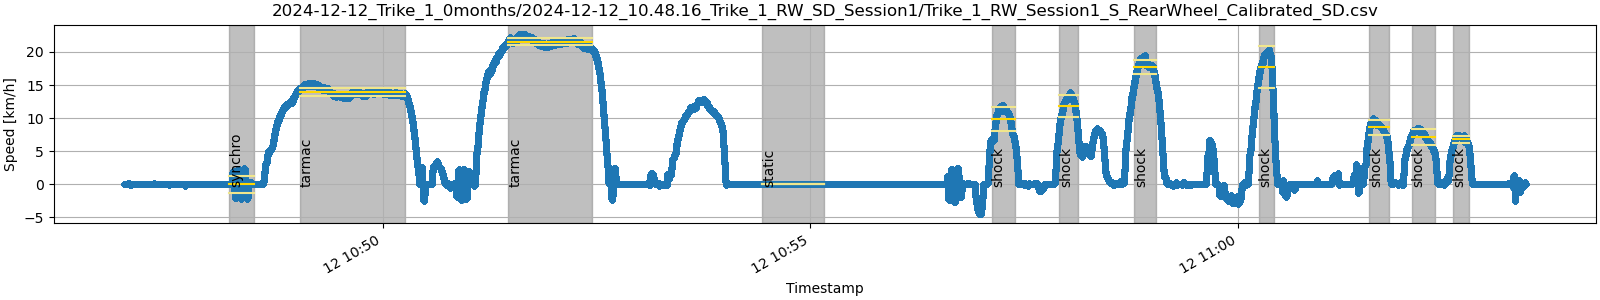
\includegraphics[width=160mm]{fig/session015.png}
  \caption{Vehicle speed versus time for an entire session (015) showing the
  segmented trials in the shaded grey areas. Gold horizontal lines depict the
  mean speed bounded by the standard deviation of the speed.}
  \label{fig:session}
\end{figure}
%
\begin{table}
  \centering
  \caption{Number of trials performed on each road surface and speed along with
  the mean duration and its standard deviation.}
\begin{tabular}{lllrrr}
\toprule
 &  &  & Count & \multicolumn{2}{c}{Duration [s]}  \\
Vehicle Type & Road Surface & Target Speed [km/h] &  & Mean & STD  \\
\midrule
\multirow[t]{6}{*}{Cargo Bicycle} & \multirow[t]{3}{*}{Tarmac} & 12 & 6 & 58.33 & 8.56 \\
 &  & 20 & 3 & 50.42 & 7.04 \\
 &  & 25 & 3 & 44.08 & 1.60 \\
\cline{2-6}
 & \multirow[t]{3}{*}{Paver Bricks} & 12 & 6 & 54.46 & 5.95 \\
 &  & 20 & 6 & 38.68 & 5.08 \\
 &  & 25 & 3 & 33.43 & 4.25 \\
\cline{1-6} \cline{2-6}
\multirow[t]{5}{*}{Stroller} & Tarmac & 5 & 10 & 27.87 & 10.07 \\
\cline{2-6}
 & Cobblestones & 5 & 13 & 27.90 & 24.74 \\
\cline{2-6}
 & Paver Bricks & 5 & 6 & 51.47 & 21.62 \\
\cline{2-6}
 & Sidewalk Slabs & 5 & 16 & 19.59 & 6.59 \\
\cline{2-6}
 & Sidewalk Pavers & 5 & 6 & 48.94 & 19.71 \\
\cline{1-6} \cline{2-6}
 & & \textbf{Count Sum} & \textbf{78} & & \\
\bottomrule
\end{tabular}
  \label{tab:num-trials}
\end{table}

\subsubsection{Trial Analyses}
%
Figure~\ref{fig:vert-acc-example} shows an example time history of the vertical
acceleration of the seat pan during a single trial. We downsampled the time
history from the set sampling frequency of 910.22~\si{\hertz} to \(N\) samples
at a constant sample rate of 400~\si{\hertz} with linear interpolation.
%
\begin{figure}
  \centering
  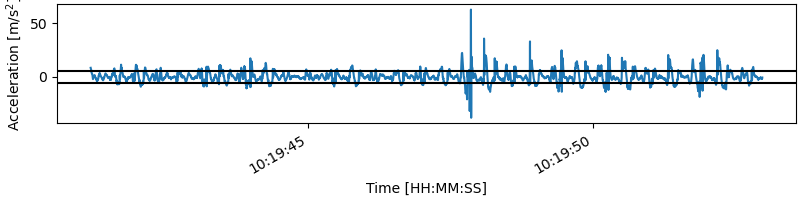
\includegraphics[width=160mm]{fig/session001-t2-aula-stroller-maxicosi-cot-0-SeatBotacc_ver.png}
  \caption{Seat pan vertical acceleration from session 1: Maxi-Cosi Stroller over
  the Sidewalk Slabs. Black horizontal lines indicate the \(\pm\)RMS
  boundary.}
  \label{fig:vert-acc-example}
\end{figure}

We calculated the root mean square of the downsampled vertical component of
acceleration at the seat pan for each trial using Equation~\ref{eq:rms-acc}.
This quantity gives an indicator of the average vertical acceleration
experienced at the baby's buttocks for the duration of the trial and can be seen
in Figure~\ref{fig:vert-acc-example}. RMS acceleration is the primary metric
recommended by ISO-2631-1 for evaluation of health and comfort in whole body
vibration.
%
\begin{align}
  \textrm{RMS}_{a_z} = \sqrt{\frac{1}{N}\sum_{n=1}^{N} a_z^2(t_n)}
  \label{eq:rms-acc}
\end{align}

We also calculated the frequency spectrum of the vertical acceleration time
history of each trial using the Fast Fourier Transform (FFT).
Figure~\ref{fig:freq-spectrum} gives an example of a frequency spectrum. In this
case, the primary peak frequency is identified to be 6.5~\si{\hertz} and the
frequency content is mostly contained below about 80~\si{\hertz}.
%
\begin{figure}
  \centering
  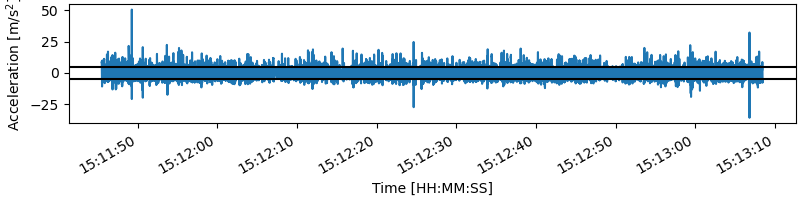
\includegraphics[width=160mm]{fig/session004-t0-pave-stroller-maxicosi-cot-0-SeatBotacc_ver.png}
  \caption{Seat pan vertical acceleration frequency spectrum from session 4:
  Maxi-Cosi Stroller over cobblestones. The gray curve shows the result of the
  FFT and the blue line is a smoothed version (Butterworth low pass
  forward/reverse). The orange vertical line indicates the frequency at the
  maximum amplitude of the smoothed curve. The green vertical line indicates the
  bandwidth threshold for 80\% of the area under the filtered curve.}
  \label{fig:freq-spectrum}
\end{figure}

\section{Results}
%
\subsection{Effect of Speed}
%
We tested the two cargo bicycles at three different target speeds: 12, 20, and
25~\si{\kilo\meter\per\hour}. Figure~\ref{fig:compare-bicycle-speed} shows the
variation in vertical RMS acceleration across the tested speeds. Accelerations
experienced when riding over the paver bricks are always larger than riding over
tarmac at the same speed, with the paver bricks having about a 5\(\times\)
increase in magnitude over tarmac. Over paver bricks, the RMS acceleration
increases by 1.7\(\times\) when increasing the speed from
\SIrange{12}{25}{\kilo\meter\per\hour}. The effect of speed while over tarmac is
less drastic but also increases over the speed range.
%
\begin{figure}
  \centering
  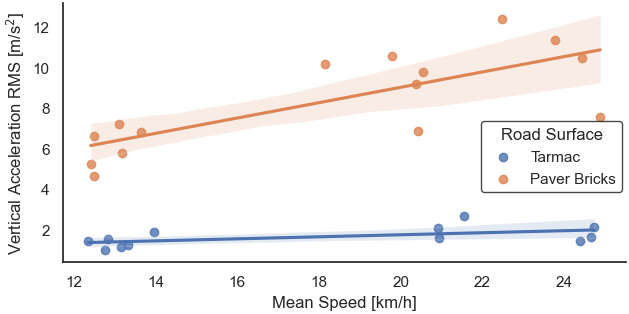
\includegraphics[width=160mm]{fig/SeatBotacc_ver-bicycle-speed-compare.png}
  \caption{Seat pan vertical acceleration RMS versus speed for all cargo bicycle
  trials. Shaded regions represent the 95\% confidence intervals from a simple
  linear regression.}
  \label{fig:compare-bicycle-speed}
\end{figure}

\subsection{Effect of Baby Size}
%
We tested dummy babies representing ages 0~months (3.5~\si{\kilo\gram}),
3~months (5.9~\si{\kilo\gram}), and 9~months (8.9~\si{\kilo\gram}).
Figure~\ref{fig:compare-baby-mass} shows the vertical RMS acceleration for each
trial for the strollers and the bicycles, comparing the baby size. There are
larger accelerations experienced in the bicycle versus the stroller, mostly
attributed to the different testing speeds. When comparing the vertical RMS
acceleration values within each vehicle type there are no obvious differences
due to baby size, i.e. each baby size experiences a similar range of
acceleration magnitudes.
%
\begin{figure}
  \centering
  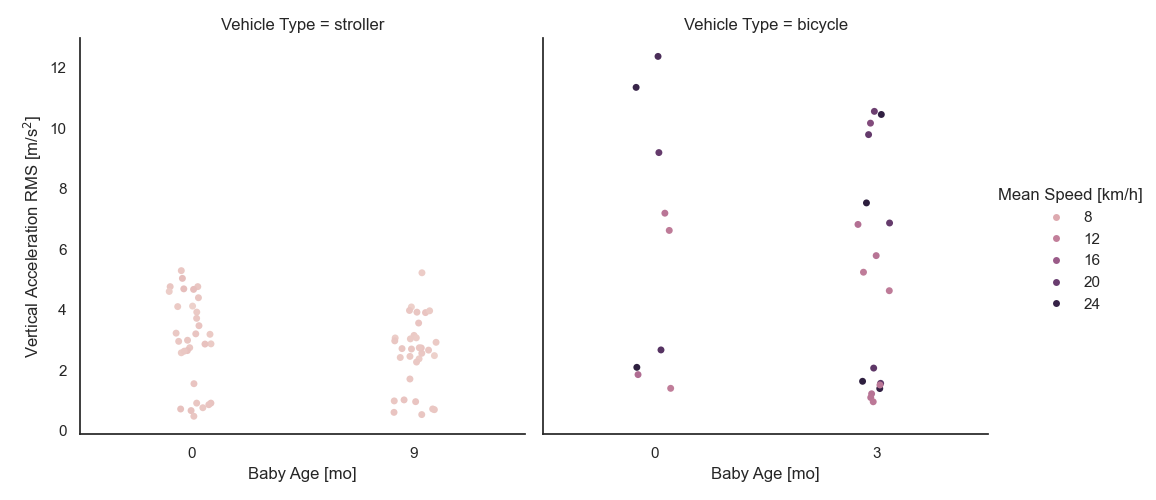
\includegraphics[width=160mm]{fig/SeatBotacc_ver-baby-mass-compare.png}
  \caption{Seat pan vertical RMS acceleration grouped by baby age (and thus size
  \& mass) for all trials with colour indicating the mean speed of the
  trial.}
  \label{fig:compare-baby-mass}
\end{figure}

\subsection{Effect of Road Surface}
%
Figure~\ref{fig:compare-road-surface} shows vertical RMS acceleration from
trials grouped into the various road surfaces we tested. All vehicles were
tested on tarmac and paver bricks but only strollers were tested on cobblestones
and sidewalks. It is notable that tarmac almost always has lower RMS
acceleration regardless of speed and vehicle type. The sidewalk slabs can have
slightly higher acceleration than cobblestones for the strollers. Paver bricks
and sidewalk pavers have a similar range of RMS acceleration for the same
5~\si{\kilo\meter\per\hour} walking speeds. Paver bricks cause relatively large
accelerations at high travel speeds in the cargo bicycles.
%
\begin{figure}
  \centering
  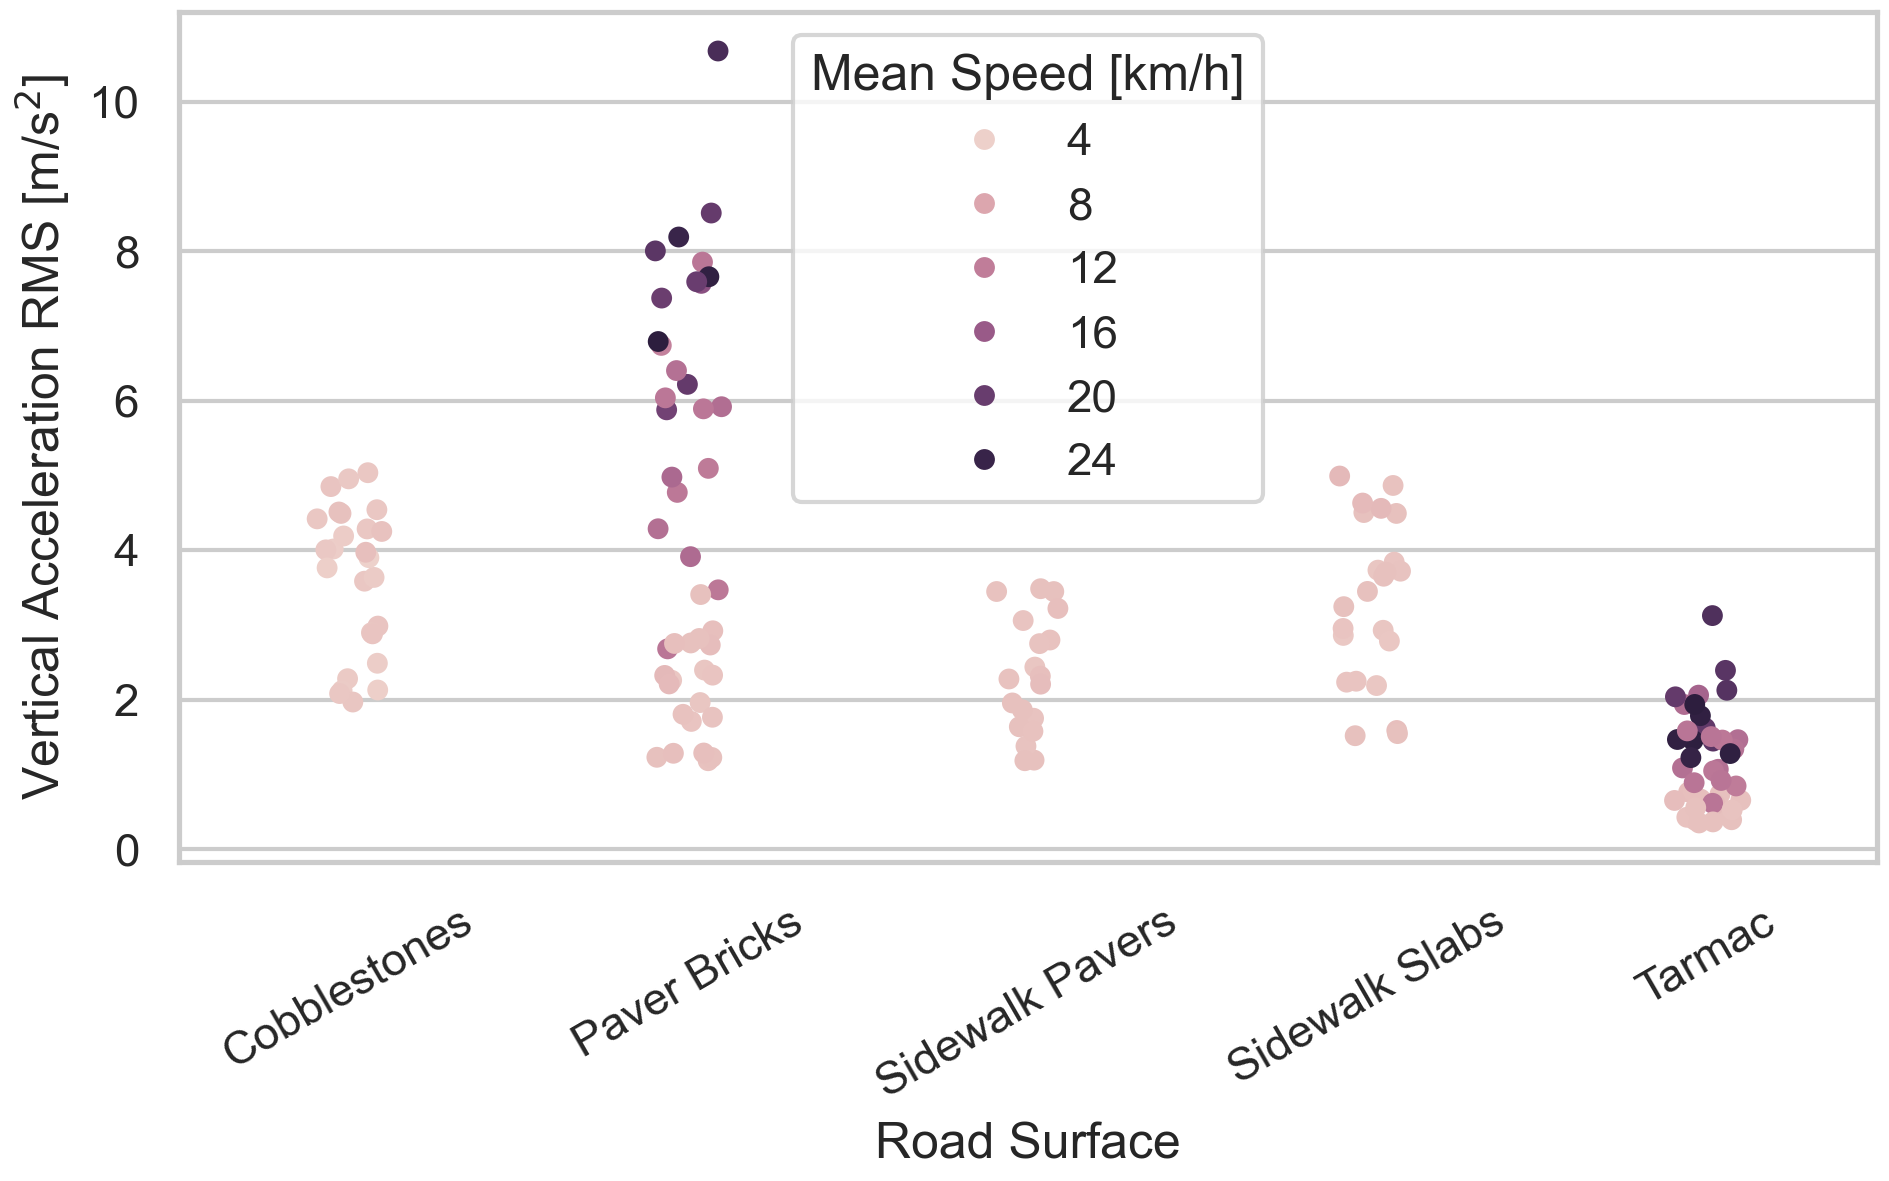
\includegraphics[width=160mm]{fig/SeatBotacc_ver-road-surface-compare.png}
  \caption{Seat pan vertical RMS acceleration grouped by road surface with
  colour indicating the mean speed of the trial. The lightest colour dots are
  strollers and the rest are cargo bicycles.}
  \label{fig:compare-road-surface}
\end{figure}

\subsection{Effect of Vehicle Model}
%
We tested three models of strollers over five different road surfaces.
Figure~\ref{fig:stroller-type-compare} compares the vertical RMS accelerations
for each road surface for each of the three strollers. The Maxi-Cosi Street Plus
and Stokke BABYZEN YOYO 0+ strollers have similar mean values across trials. The
Bugaboo has a slightly lower mean, but much larger variation in the RMS values.
There may be no significant difference in the acceleration experienced in each
stroller model. All road surfaces compared to tarmac cause at least double the
RMS acceleration.
%
\begin{figure}
  \centering
  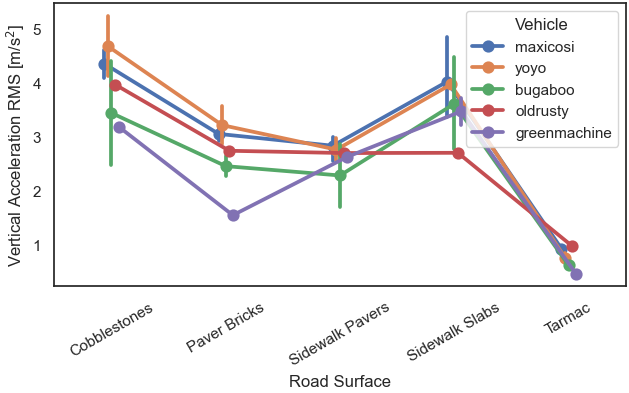
\includegraphics[width=160mm]{fig/SeatBotacc_ver-stroller-type-compare.png}
  \caption{Mean seat pan vertical RMS acceleration per road surface for each
  stroller. Vertical lines indicate the standard deviation for categories that
  have more than one trial.} 
  \label{fig:stroller-type-compare}
\end{figure}

Figure~\ref{fig:bicycle-type-compare} compares the two cargo bicycle models we
tested. Each cargo bicycle was fitted with the same set of two baby seats (Melia
baby shell and Maxi-Cosi Pebble Pro baby seat). The two-wheel cargo bicycle
seems to deliver lower acceleration to the seat pan, but the variation in the
data is large, indicating there may be no significant difference between the two
vehicles. Both vehicles show increasing vertical RMS acceleration with speed.
%
\begin{figure}
  \centering
  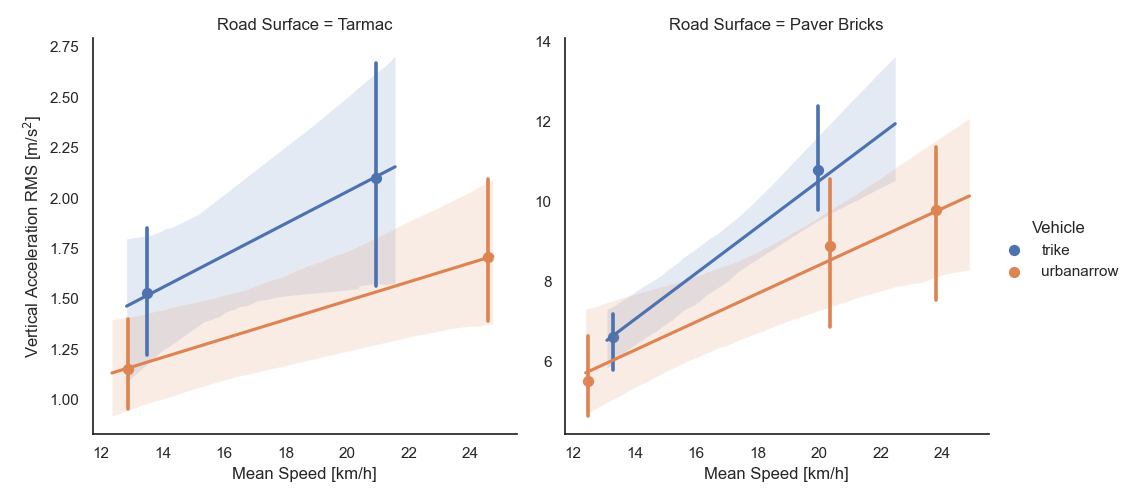
\includegraphics[width=160mm]{fig/SeatBotacc_ver-bicycle-type-compare.png}
  \caption{Seat pan vertical RMS acceleration versus speed grouped by road
  surface and cargo bicycle model. Horizontal lines indicate a linear
  regression, vertical lines are the standard deviation at those speeds, and
  shaded regions show the 95\% confidence intervals for the regression.}
  \label{fig:bicycle-type-compare}
\end{figure}

\subsection{Dominant Frequency and Bandwidth}
%
Figure~\ref{fig:peak-freq-dist} shows the dominant frequency compared among road
surface types for each of the target speeds. Peak frequencies range from
\SIrange{5}{11}{\hertz} across all trials. For strollers
(5~\si{\kilo\meter\per\hour}, the median frequency increases from sidewalk
slabs, to cobblestones, to sidewalk pavers, to tarmac, to paver bricks. With the
exception of paver bricks being larger than tarmac this increase corresponds to
an increase in the size of the geometric surface features of the road.
%
\begin{figure}
  \centering
  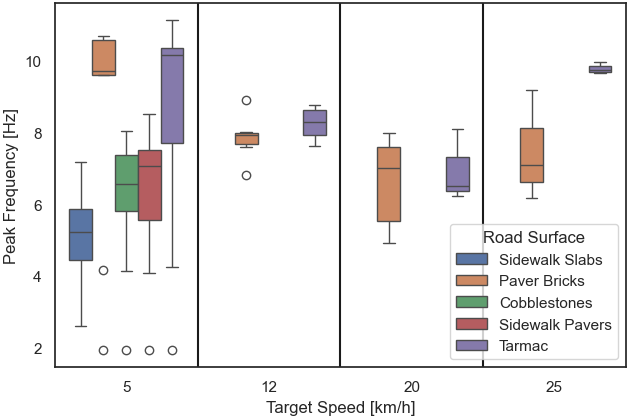
\includegraphics[width=160mm]{fig/SeatBotacc_ver-peak-freq-dist.png}
  \caption{Peak frequency distributions comparisons among road surfaces for each
  target speed group. The boxes bound the quartiles and indicate the median. The
  whiskers indicate the 95th perentile and circles are any outliers.}
  \label{fig:peak-freq-dist}
\end{figure}

Figure~\ref{fig:thresh-freq-dist} gives a general indication of bandwidth
distributions for each of the target speed groups. Most frequency content is
below 100~\si{\hertz} for the all trials. The median threshold frequency across
all trials is 70~\si{\hertz} which gives an idea of the bandwidth for the
vibrations of interest.
%
\begin{figure}
  \centering
  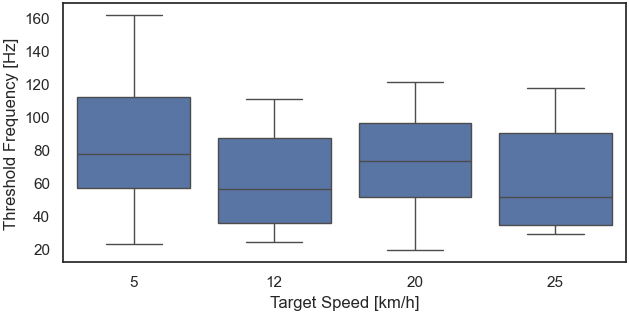
\includegraphics[width=160mm]{fig/SeatBotacc_ver-thresh-freq-dist.png}
  \caption{Threshold frequency  (based on 80\% of the area under the filtered
  frequency spectrum) for each target speed group.}
  \label{fig:thresh-freq-dist}
\end{figure}

\subsection{Overall Comparison}
We tabulate the seat pan vertical RMS acceleration, trial duration, peak
frequency, and threshold frequency for all 52 combinations of vehicle setup,
road surface, and target speed in Table~\ref{tab:results}.
Figure~\ref{fig:compare-all} shows the vertical RMS acceleration of all trials
broken down by vehicle setup (vehicle, seat, baby age), road surface, trial
duration, and travel speed. Some additional insights can be gathered from this
figure, that are not seen in the prior figures.
%
\begin{itemize}
    \item The baby in stroller travelling at 5~\si{\kilo\meter\per\hour} over
    cobblestones and sidewalks slabs cracks can experience accelerations of
    similar magnitude to a baby in a cargo bicycle travelling at
    12~\si{\kilo\meter\per\hour} over paver bricks.
    \item A 3 month old baby in a baby shell (Melia) travelling over brick
    pavers at high speeds has lower RMS acceleration than the same baby in a car
    seat (Maxi-Cosi Pebble Pro) in the Urban Arrow and it may also be true for
    the Keiler tricycle. Switching to the baby shell in the Urban Arrow has a
    similar effect to reducing speed by 10~\si{\kilo\meter\per\hour}.
\end{itemize}

\begin{table}
  \centering
  \caption{Computed metrics for all 52 scenarios measured.}
  \label{tab:results}
  \footnotesize
\begin{tabular}{lllcccccc}
\toprule
        &            &              &        &       & Mean         &          & Mean      & Mean      \\
Vehicle & Seat, Baby & Road Surface & Target & Trial & RMS          & Mean     & Peak      & Threshold \\
        &            &              & Speed  & Count & Acceleration & Duration & Frequency & Frequency \\
        &            &              & [km/h] &       &  [m/s\(^2\)]     & [s]      & [Hz]      & [Hz]      \\
\midrule
\multirow[t]{10}{*}{bugaboo} & \multirow[t]{5}{*}{cot, 0 mo} & Cobblestones & 5 & 2 & 4.4 & 39.8 & 6.6 & 22.6 \\
\cline{3-9}
 &  & Paver Bricks & 5 & 1 & 2.6 & 70.5 & 10.7 & 25.1 \\
\cline{3-9}
 &  & Sidewalk Pavers & 5 & 1 & 2.9 & 51.6 & 8.2 & 119.5 \\
\cline{3-9}
 &  & Sidewalk Slabs & 5 & 3 & 4.8 & 20.0 & 5.8 & 41.8 \\
\cline{3-9}
 &  & Tarmac & 5 & 2 & 0.7 & 24.9 & 9.9 & 61.5 \\
\cline{2-9} \cline{3-9}
 & \multirow[t]{5}{*}{seat, 9 mo} & Cobblestones & 5 & 2 & 2.5 & 42.0 & 6.8 & 46.5 \\
\cline{3-9}
 &  & Paver Bricks & 5 & 1 & 2.3 & 66.9 & 9.7 & 57.5 \\
\cline{3-9}
 &  & Sidewalk Pavers & 5 & 1 & 1.7 & 71.3 & 7.6 & 47.4 \\
\cline{3-9}
 &  & Sidewalk Slabs & 5 & 3 & 2.4 & 23.9 & 6.0 & 47.1 \\
\cline{3-9}
 &  & Tarmac & 5 & 2 & 0.6 & 33.2 & 8.4 & 68.9 \\
\cline{1-9} \cline{2-9} \cline{3-9}
\multirow[t]{10}{*}{maxicosi} & \multirow[t]{5}{*}{cot, 0 mo} & Cobblestones & 5 & 1 & 4.6 & 81.7 & 6.6 & 82.3 \\
\cline{3-9}
 &  & Paver Bricks & 5 & 1 & 3.2 & 61.5 & 10.6 & 75.6 \\
\cline{3-9}
 &  & Sidewalk Pavers & 5 & 1 & 3.0 & 51.0 & 7.8 & 79.7 \\
\cline{3-9}
 &  & Sidewalk Slabs & 5 & 5 & 4.5 & 12.3 & 5.7 & 80.3 \\
\cline{3-9}
 &  & Tarmac & 5 & 2 & 0.9 & 29.4 & 10.5 & 56.5 \\
\cline{2-9} \cline{3-9}
 & \multirow[t]{5}{*}{seat, 9 mo} & Cobblestones & 5 & 5 & 4.2 & 12.6 & 7.8 & 65.8 \\
\cline{3-9}
 &  & Paver Bricks & 5 & 2 & 3.0 & 26.0 & 9.8 & 79.6 \\
\cline{3-9}
 &  & Sidewalk Pavers & 5 & 1 & 2.6 & 54.8 & 6.8 & 67.1 \\
\cline{3-9}
 &  & Sidewalk Slabs & 5 & 3 & 3.2 & 23.0 & 6.9 & 70.4 \\
\cline{3-9}
 &  & Tarmac & 5 & 2 & 1.0 & 33.6 & 10.2 & 70.7 \\
\cline{1-9} \cline{2-9} \cline{3-9}
\multirow[t]{12}{*}{trike} & \multirow[t]{4}{*}{maxicosi, 0 mo} & \multirow[t]{2}{*}{Paver Bricks} & 12 & 1 & 7.2 & 47.6 & 8.0 & 44.9 \\
 &  &  & 20 & 1 & 11.1 & 35.3 & 6.4 & 101.6 \\
\cline{3-9}
 &  & \multirow[t]{2}{*}{Tarmac} & 12 & 1 & 1.9 & 73.7 & 8.1 & 23.8 \\
 &  &  & 20 & 1 & 2.7 & 58.4 & 6.5 & 18.8 \\
\cline{2-9} \cline{3-9}
 & \multirow[t]{4}{*}{maxicosi, 3 mo} & \multirow[t]{2}{*}{Paver Bricks} & 12 & 1 & 6.8 & 57.8 & 7.9 & 72.3 \\
 &  &  & 20 & 1 & 9.8 & 42.8 & 7.1 & 87.2 \\
\cline{3-9}
 &  & \multirow[t]{2}{*}{Tarmac} & 12 & 1 & 1.5 & 55.6 & 7.6 & 31.7 \\
 &  &  & 20 & 1 & 2.1 & 47.6 & 6.2 & 19.2 \\
\cline{2-9} \cline{3-9}
 & \multirow[t]{4}{*}{melia, 3 mo} & \multirow[t]{2}{*}{Paver Bricks} & 12 & 1 & 5.8 & 52.6 & 8.9 & 100.5 \\
 &  &  & 20 & 1 & 10.2 & 46.0 & 6.9 & 120.9 \\
\cline{3-9}
 &  & \multirow[t]{2}{*}{Tarmac} & 12 & 1 & 1.2 & 50.8 & 7.9 & 91.1 \\
 &  &  & 20 & 1 & 1.6 & 45.2 & 8.1 & 72.8 \\
\cline{1-9} \cline{2-9} \cline{3-9}
\multirow[t]{15}{*}{urbanarrow} & \multirow[t]{5}{*}{maxicosi, 0 mo} & \multirow[t]{3}{*}{Paver Bricks} & 12 & 1 & 6.6 & 62.3 & 7.6 & 110.4 \\
 &  &  & 20 & 1 & 9.2 & 39.1 & 8.0 & 71.6 \\
 &  &  & 25 & 1 & 11.4 & 38.3 & 7.1 & 117.5 \\
\cline{3-9}
 &  & \multirow[t]{2}{*}{Tarmac} & 12 & 1 & 1.4 & 58.1 & 8.7 & 28.9 \\
 &  &  & 25 & 1 & 2.1 & 43.1 & 10.0 & 28.5 \\
\cline{2-9} \cline{3-9}
 & \multirow[t]{5}{*}{maxicosi, 3 mo} & \multirow[t]{3}{*}{Paver Bricks} & 12 & 1 & 5.2 & 58.2 & 7.9 & 85.7 \\
 &  &  & 20 & 1 & 10.6 & 32.1 & 4.9 & 102.8 \\
 &  &  & 25 & 1 & 10.5 & 30.3 & 6.2 & 99.3 \\
\cline{3-9}
 &  & \multirow[t]{2}{*}{Tarmac} & 12 & 1 & 1.1 & 50.7 & 8.8 & 37.8 \\
 &  &  & 25 & 1 & 1.6 & 43.2 & 9.6 & 31.8 \\
\cline{2-9} \cline{3-9}
 & \multirow[t]{5}{*}{melia, 3 mo} & \multirow[t]{3}{*}{Paver Bricks} & 12 & 1 & 4.6 & 48.3 & 6.8 & 36.6 \\
 &  &  & 20 & 1 & 6.9 & 36.8 & 7.8 & 51.1 \\
 &  &  & 25 & 1 & 7.5 & 31.7 & 9.2 & 60.6 \\
\cline{3-9}
 &  & \multirow[t]{2}{*}{Tarmac} & 12 & 1 & 1.0 & 61.2 & 8.5 & 66.5 \\
 &  &  & 25 & 1 & 1.4 & 45.9 & 9.7 & 41.7 \\
\cline{1-9} \cline{2-9} \cline{3-9}
\multirow[t]{5}{*}{yoyo} & \multirow[t]{5}{*}{cot, 0 mo} & Cobblestones & 5 & 3 & 4.1 & 18.1 & 6.6 & 91.1 \\
\cline{3-9}
 &  & Paver Bricks & 5 & 1 & 2.8 & 57.8 & 9.7 & 123.9 \\
\cline{3-9}
 &  & Sidewalk Pavers & 5 & 2 & 2.6 & 32.5 & 6.5 & 98.9 \\
\cline{3-9}
 &  & Sidewalk Slabs & 5 & 2 & 4.0 & 25.7 & 5.1 & 103.8 \\
\cline{3-9}
 &  & Tarmac & 5 & 2 & 0.8 & 18.1 & 7.4 & 156.6 \\
\cline{1-9} \cline{2-9} \cline{3-9}
\bottomrule
\end{tabular}
\end{table}

\begin{figure}
  \centering
  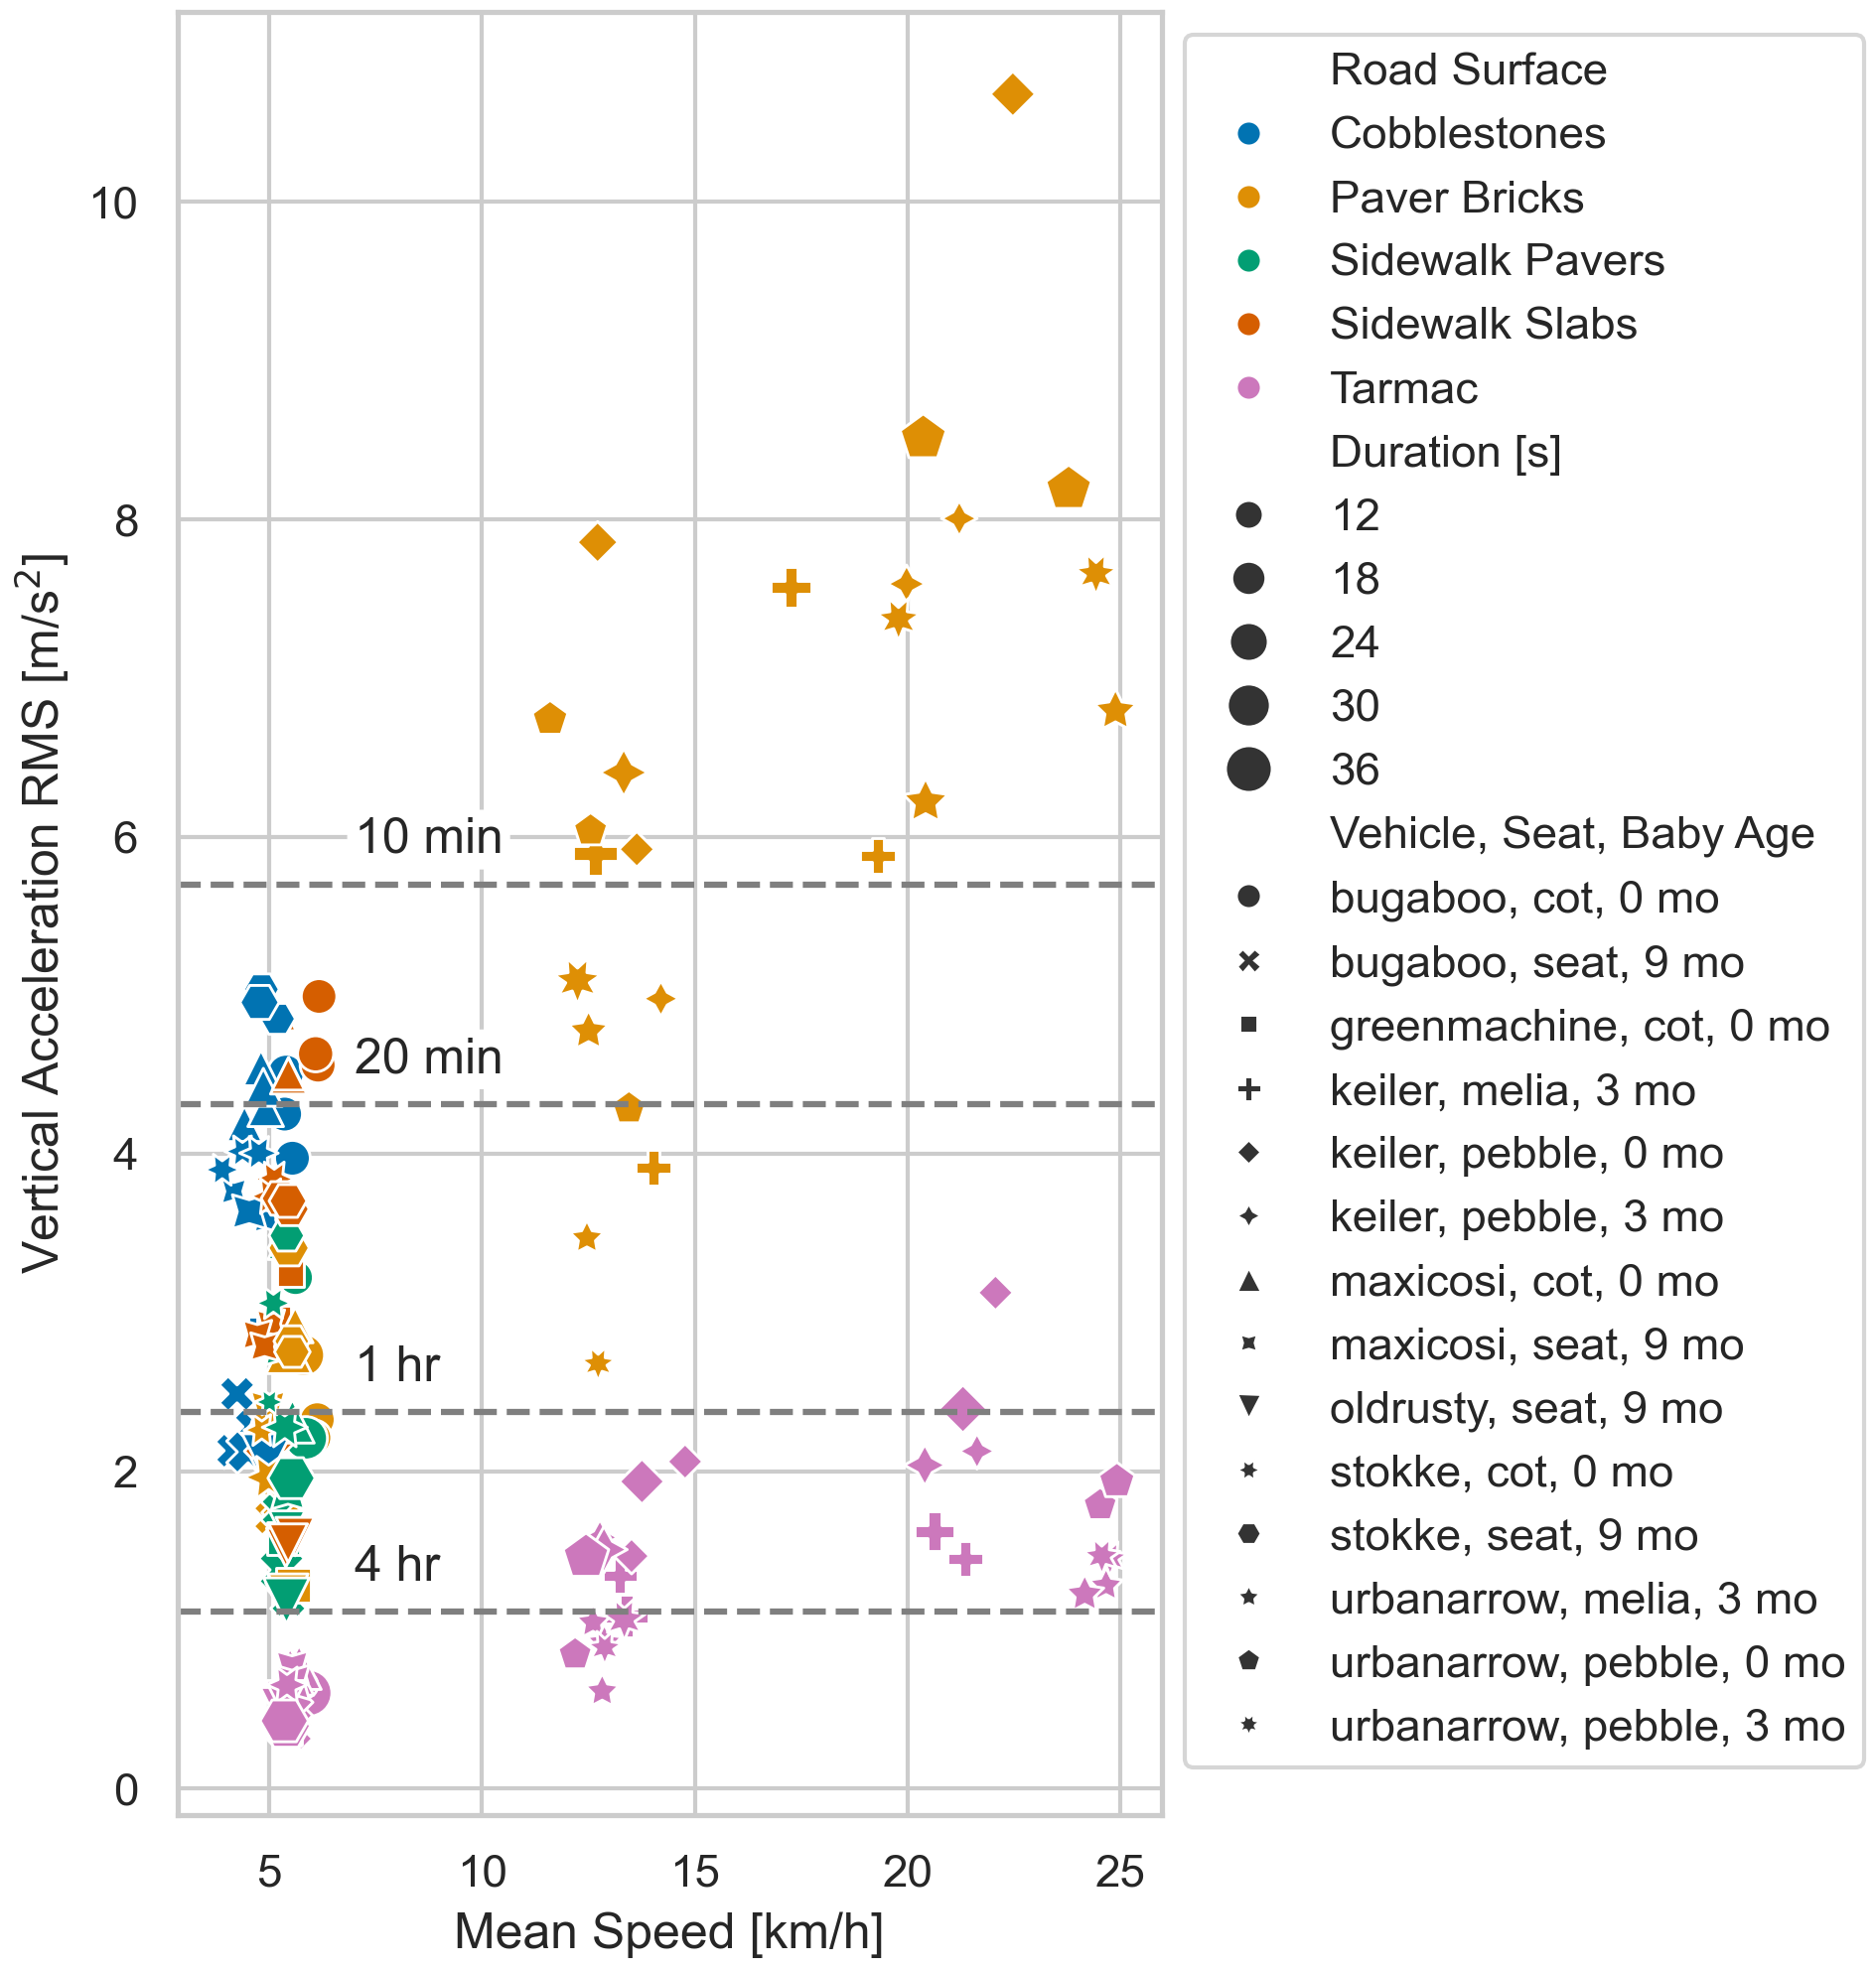
\includegraphics[width=160mm]{fig/SeatBotacc_ver-compare-all.png}
  \caption{Scatter plot of the vertical RMS acceleration of all trials broken
  down by vehicle setup, trial duration, road surface, and plotted versus
  speed.}
  \label{fig:compare-all}
\end{figure}

\section{Conclusion}
%
We have presented a comprehensive set of acceleration measurements from
experiments that simulate the vibrations experienced by babies in the 0-9 month
age range during transportation via strollers and cargo bicycles. We compare the
average magnitude of vertical acceleration at the seat pan across a variety of
road surfaces and seats while moving at typical vehicle travel speeds. In this
preliminary analysis, we report on the variation among the various independent
variables, finding that average acceleration can be relatively large for some
scenarios. We only report the characterization of the accelerations experienced
by the baby and do not weigh in on whether these can cause discomfort or have
negative health consequences. There is a large gap in the literature connecting
acceleration magnitude to discomfort and/or health consequences.

We show that average acceleration can range from
\SIrange{0.5}{11.4}{\meter\per\second\squared} across all tested scenarios.
Strollers experience \SIrange{0.5}{5.3}{\meter\per\second\squared} average
acceleration for a mean walking speed of 5.2~\si{\kilo\meter\per\hour}. Cargo
bicycles experience \SIrange{1.0}{11.4}{\meter\per\second\squared} over a speed
range of \SIrange{12}{25}{\kilo\meter\per\hour}.

Travelling over a tarmac surface offers the least vibration to all vehicle types
at any speed with a maximum average acceleration of
2.7~\si{\meter\per\second\squared}. For strollers, travelling over surfaces
rougher than tarmac at normal walking speed can cause from 1.6\(\times\) to
6.6\(\times\) the accelerations experienced on tarmac with average accelerations
reaching 5.3~\si{\meter\per\second\squared}. Cobblestones and the large gaps of
the sidewalk slabs cause the largest magnitude vibrations to the baby in the
strollers. For cargo bicycles, travelling over paver bricks at the same speeds
can quadruple the magnitude of the average acceleration the baby experiences.
Travelling at the maximum allowed speed of an electric cargo bike (25
\si{\kilo\meter\per\hour}) over paver bricks causes the baby to experience
average accelerations exceeding 8~\si{\meter\per\second\squared}. The effect of
speed on vibration is higher for paver bricks than tarmac.

The size of the baby (mass and shape) has no obvious effect on the average
accelerations experienced at the seat pan body-seat interface. These vibrations
are transmitted to the baby's body and the physical properties (mass, stiffness,
damping) of the baby's body determine whether this excitation is amplified or
not and to which body segment is more affected. Tests with more realistic
dummies or real babies is necessary to know how the baby itself moves when
excited by this level of vibration. This information is not readily available in
the literature and may be hard to perform due to ethical limitations and absence
of realistic dummies.

When comparing stroller and cargo bicycle vehicle setups (vehicle, seat, baby
age) among each other, the preliminary results show no obvious differences in
the acceleration experienced by the baby other than the baby shell being better
than a baby car seat for the 3 month old baby in the cargo bike at the maximum
speeds. This may be attributed to the suspended mounting location of the baby
seat in the cargo bay versus the baby shell being mounted to the existing bench
in the cargo bay. Statistical analysis may reveal more nuance differences among
the vehicle setups.

We also investigated the dominant frequency and bandwidth of vibrations across
the various scenarios. Vibrations at frequencies between
\SIrange{4.9}{10.7}{\hertz} have the largest magnitude contribution to the
vibrations but there is frequency content of magnitudes of interest in a
bandwidth of up to 100~\si{\hertz}.

We measured four other sensors on the vehicles, all with six accelerometer and
gyroscope time histories, for a total of 30 time histories of possible interest.
This paper provides a look into the experiments via three metrics: vertical RMS
acceleration, peak frequency, and bandwidth of effectively one of the 30 time
histories. There are a variety of other metrics that can provide insight, for
example vibration dosage value and crest factor that characterize peak
accelerations or ISO 2631-1 weighted linear and rotational accelerations that
have more connection to experienced comfort. Future work will investigate these
more closely as well as shock effects and apply standard statistical models to
the data to make more definitive conclusions in the scenario comparisons.

\bibliographystyle{plain}
\bibliography{reference}

\end{document}